%%%%%%%%%%%%%%%%%%%%%%%%%%%%%%%%%%%%%%%%%%%%%%%%%%%%%%%%%%%%%%%%%%%%%%%
% Slides for the TechCon 2022 talk "PyAnsys tools for unit testing" 
%%%%%%%%%%%%%%%%%%%%%%%%%%%%%%%%%%%%%%%%%%%%%%%%%%%%%%%%%%%%%%%%%%%%%%%
\documentclass[t]{beamer}

\usetheme{Ansys2022}

\usepackage{minted}
\usepackage{xcolor}
\usepackage{pdfpages}
\usepackage{listings}
\usepackage{tikz}
\usepackage{hyperref}

\usepackage[edges]{forest}
\hypersetup{
    colorlinks=true,
    linkcolor=blue,
    filecolor=magenta,      
    urlcolor=cyan,
}
 

\urlstyle{same}
\setbeamercolor{background canvas}{bg=}

\definecolor{bleudefrance}{rgb}{0.19, 0.55, 0.91}

%%%%%%%%%%%%%%%%%%%%%%%%%%%%%%%%%%%%%%%%%%%%%%%%%%%%%%%%%%%%%%%%%%%%%%%%%%%%%%%
\usetikzlibrary{shapes.geometric, arrows,positioning}

\tikzset{
  startstop/.style={
    rectangle, 
    rounded corners,
    minimum width=3cm,
    minimum height=0.75cm,
    align=center, 
    draw=black, 
    fill=ANSYS@Gold,
    },
  process/.style={
    rectangle, 
    minimum width=3cm, 
    minimum height=0.75cm, 
    align=center, 
    draw=black, 
    fill=ANSYS@Blue,
    text=white,
    },
  decision/.style={
    diamond, 
    aspect=4,
    minimum width=3cm, 
    minimum height=1cm,
    align=center,
    draw=black, 
    fill=ANSYS@Blue,
    text=white,
    },
  arrow/.style={thick,->,>=stealth},
  dec/.style={
    ellipse, 
    align=center, 
    draw=black, 
    fill=ANSYS@Bronze,
    },
}

\begin{document}

%%%%%%%%%%%%%%%%%%%%%%%%%%%%%%%%%%%%%%%%%%%%%%%%%%%%%%%%%%%%%%%%%%%%%%%%%%%%%%%
%% Title Slide

\title{PyAnsys tools for unit testing}
\subtitle{Applying test driven development}
\author{Author: PyAnsys Core Team}
\date{\today}

\titleframe{}


%%%%%%%%%%%%%%%%%%%%%%%%%%%%%%%%%%%%%%%%%%%%%%%%%%%%%%%%%%%%%%%%%%%%%%%%%%%%%%%
%% Table of contents

\begin{frame}{Table of Contents}
  \tableofcontents
  \vspace{200pt}  %% force top left  
\end{frame}


%%%%%%%%%%%%%%%%%%%%%%%%%%%%%%%%%%%%%%%%%%%%%%%%%%%%%%%%%%%%%%%%%%%%%%%%%%%%%%%
\section{Using this Theme}
\begin{frame}[fragile=singleslide]
  \frametitle{Using this Theme}

  \begin{itemize}

  \item{\textbf{Installation}
    
    On Linux, you'll need to install LaTeX and
    \href{https://www.luatex.org/}{LuaTeX}. On Ubuntu you can do this with:

    \begin{lstlisting}[language=bash,basicstyle=\footnotesize\ttfamily]
sudo apt update
sudo apt install -y latexmk texlive-luatex texlive-fonts-extra
    \end{lstlisting}


    On Windows, follow the directions at
    \href{https://www.latex-project.org/get/}{Getting LaTeX} and download the
    \href{HTTP://www.tug.org/texlive}{TeX Live} distribution. It's the easiest
    way to get started.
  }

  \item{\textbf{Building}

    Build a PDF from the text file with:

    \begin{lstlisting}[language=bash,basicstyle=\footnotesize\ttfamily]
latexmk -pdflatex=lualatex -pdf sample.tex -interaction=nonstopmode -outdir=./build
    \end{lstlisting}

    }

  \end{itemize}

\end{frame}

%%%%%%%%%%%%%%%%%%%%%%%%%%%%%%%%%%%%%%%%%%%%%%%%%%%%%%%%%%%%%%%%%%%%%%%%%%%%%%%
\section{Slide Types}

\begin{frame}
  \frametitle{Content}
  \tableofcontents[currentsection]
  \vspace{200pt}  %% force top left
\end{frame}


\subsection{Basic Slide}
\begin{frame}[fragile=singleslide]  % must use fragile with any input listing
  \frametitle{Basic Slide}

  A basic slide consists of:

  \lstinputlisting[basicstyle=\footnotesize\ttfamily]{code/slideframe.tex}

  The output from the above source is the following slide.

\end{frame}

\begin{frame}
  \frametitle{This is the Frame Title}
  
  This is a basic frame. Bulleted lists can be created with:
  \begin{itemize}
    \item{Item A}
    \item{Item B}
    \item{Item C}
  \end{itemize}

\end{frame}


%%%%%%%%%%%%%%%%%%%%%%%%%%%%%%%%%%%%%%%%%%%%%%%%%%%%%%%%%%%%%%%%%%%%%%%%%%%%%%%
\subsection{Transition Slide}
\begin{frame}[fragile=singleslide]
  \frametitle{Transition Slide}

  A transition slide can be created with:
  \vspace{\baselineskip}

  \verb|\textbackslash transitionframe{Transition slide text}|
  \vspace{\baselineskip}

  Note how \verb|The [fragile=singleslide]|option is used when using verbatim
  text within this slide.
  \vspace{\baselineskip}

  Transition slide follows.

\end{frame}

\transitionframe{Transition slide text}

%%%%%%%%%%%%%%%%%%%%%%%%%%%%%%%%%%%%%%%%%%%%%%%%%%%%%%%%%%%%%%%%%%%%%%%%%%%%%%%
\subsection{End Slide}
\begin{frame}[fragile=singleslide]
  \frametitle{End Slide}

  The end slide can be created with:
  \vspace{\baselineskip}

  \verb|\lastframe|
  \vspace{\baselineskip}

  The end slide follows.

\end{frame}

\lastframe{}

%%%%%%%%%%%%%%%%%%%%%%%%%%%%%%%%%%%%%%%%%%%%%%%%%%%%%%%%%%%%%%%%%%%%%%%%%%%%%%%
\section{LaTeX Beamer Features}

\begin{frame}
  \frametitle{LaTeX Beamer Features}
  \tableofcontents[currentsection]
  \vspace{200pt}  %% force top left
\end{frame}

\begin{frame}[fragile=singleslide]
  \frametitle{LaTeX Beamer Features}

  The Beamer document class contains a variety of features to simplify creating
  presentations within LaTeX. This includes:

  \begin{itemize}
    \item{Title Page}
    \item{Table of Contents}
    \item{Blocks}
  \end{itemize}

  For more details, see
  \href{https://www.overleaf.com/learn/latex/Beamer}{Overleaf - Beamer}.

\end{frame}

%%%%%%%%%%%%%%%%%%%%%%%%%%%%%%%%%%%%%%%%%%%%%%%%%%%%%%%%%%%%%%%%%%%%%%%%%%%%%%%
\subsection{Title Slide}
\begin{frame}[fragile=singleslide]
  \frametitle{Title Slide}

  The title slide uses the \verb|\titleframe{}| command preceded by commands
  containing metadata of the presentation.

  \begin{lstlisting}[basicstyle=\footnotesize\ttfamily]

\title{Title}
\subtitle{Subtitle (optional)}
\author{First Middle Last}
\date{\today}

  \end{lstlisting}

\end{frame}

%%%%%%%%%%%%%%%%%%%%%%%%%%%%%%%%%%%%%%%%%%%%%%%%%%%%%%%%%%%%%%%%%%%%%%%%%%%%%%%
\subsection{Table of Contents}
\begin{frame}[fragile=singleslide]
  \frametitle{Title Slide}

  You can auto-generate a table of contents using the \verb|\tableofcontents|
  command. For example:

  \begin{lstlisting}[basicstyle=\footnotesize\ttfamily]
\begin{frame}{Table of Contents}
  \tableofcontents
  \vspace{200pt}  %% force top left  
\end{frame}
  \end{lstlisting}

  This table of contents will be built off of the standard \verb|\section| and
  \verb|\subsection| used to organize your presentation. These should precede
  key slides right before \verb|\begin{frame}|.

  \begin{lstlisting}[basicstyle=\footnotesize\ttfamily]
\section{Problem statement}
\section{Existing results}
    \subsection{Method 1}
    \subsection{Method 2}
\section{Comparative study}
  \end{lstlisting}

\end{frame}

%%%%%%%%%%%%%%%%%%%%%%%%%%%%%%%%%%%%%%%%%%%%%%%%%%%%%%%%%%%%%%%%%%%%%%%%%%%%%%%
\subsection{Blocks}
\begin{frame}
  \frametitle{Blocks}

  Blocks can be used to highlight important points within a presentation.

  \begin{block}{Default Block}
    Block text.
  \end{block}

  \begin{alertblock}{Alert Block}
    Block text in an alert block.
  \end{alertblock}

  \begin{examples}
    Block text in Ansys Gold block.
  \end{examples}

\end{frame}


%%%%%%%%%%%%%%%%%%%%%%%%%%%%%%%%%%%%%%%%%%%%%%%%%%%%%%%%%%%%%%%%%%%%%%%%%%%%%%%
\section{Content}

\begin{frame}
  \frametitle{Content}
  \tableofcontents[currentsection]
  \vspace{200pt}  %% force top left
\end{frame}


\begin{frame}
  \frametitle{Content}
  Content in a Beamer presentation can come in a variety of forms, including:

  \begin{itemize}
    \item{Figures}
    \item{Flowcharts}
    \item{Code}
  \end{itemize}

  The following slides provide several examples for how you can include content
  in a LaTeX presentation.

\end{frame}

%%%%%%%%%%%%%%%%%%%%%%%%%%%%%%%%%%%%%%%%%%%%%%%%%%%%%%%%%%%%%%%%%%%%%%%%%%%%%%%
\subsection{Figures}
\begin{frame}
  \frametitle{Figures - Full Slide}
  \vspace{-10pt}

  Figures can be made to take up most of the slide:

  \centering
  
\includegraphics[height=.7\textheight]{./figures/github.png}

\end{frame}


%%%%%%%%%%%%%%%%%%%%%%%%%%%%%%%%%%%%%%%%%%%%%%%%%%%%%%%%%%%%%%%%%%%%%%%%%%%%%%%
\begin{frame}[fragile=singleslide]
  \frametitle{Figures - Using Tabular}
  \vspace{-10pt}

  Figures can also be made to fit alongside text content using either tables or
  columns. Here we demonstrate using tables with the figure on the left.

  \vspace{6pt}

  \begin{tabular}{cl}  
    \begin{tabular}{c}
      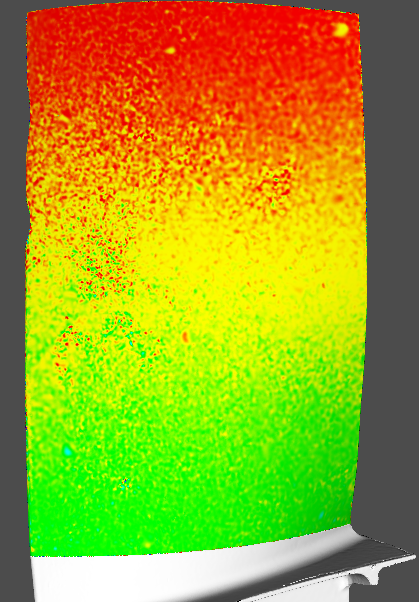
\includegraphics[height=5cm, width=3.5cm]{figures/blade_accuracy.png}
    \end{tabular}
    & \begin{tabular}{r}
        \parbox{0.7\linewidth}{
            \begin{itemize}
            \item{Item A}
            \item{Item B}
            \item{Item C}
            \end{itemize}
        }
      \end{tabular}  \\
\end{tabular}

\end{frame}


%%%%%%%%%%%%%%%%%%%%%%%%%%%%%%%%%%%%%%%%%%%%%%%%%%%%%%%%%%%%%%%%%%%%%%%%%%%%%%%
\begin{frame}[fragile=singleslide]
  \frametitle{Figures - Using Columns}
  \vspace{-10pt}

  Here we demonstrate showing a figure using two columns with code on the left
  and the figure on the right.

  \hrulefill{}

  \begin{columns}[T]
    \begin{column}{.5\textwidth}
      \vspace{-5pt}
      \inputminted[fontsize=\footnotesize]{python}{code/sample_mpl.py}
    \end{column}

    \begin{column}{.5\textwidth}          
      %% \begin{figure}
      \centering
      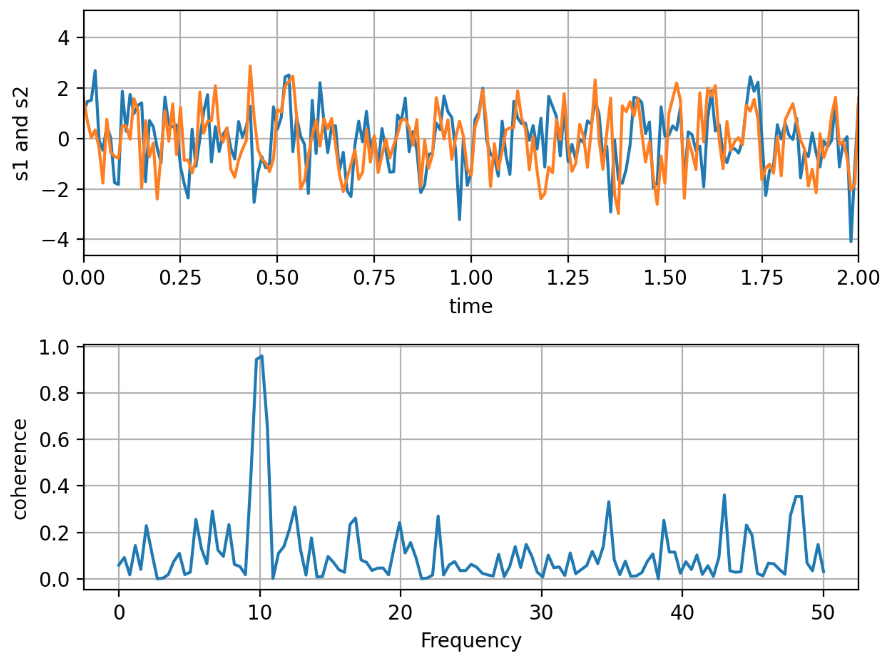
\includegraphics[height=5cm]{figures/sample_mpl.png}
      %% \end{figure}
    \end{column}

  \end{columns}

\end{frame}


%%%%%%%%%%%%%%%%%%%%%%%%%%%%%%%%%%%%%%%%%%%%%%%%%%%%%%%%%%%%%%%%%%%%%%%%%%%%%%%
\subsection{Flowchart}
\begin{frame}
  \frametitle{Example Flowchart}
  \vspace{-10pt}

    \begin{columns}[T]
        \begin{column}{.6\textwidth}
          \begin{itemize}
            \item This is a two column slide with a sample flowchart on the right.
            \item This flowchart uses the edges package.
            \item This two column format is helpful when including figures and
              text in the same page.
          \end{itemize}
        \end{column}


        \begin{column}{.4\textwidth}          
          \begin{figure}
            \centering
            \begin{forest}
              for tree={
                draw,
                align=center
              },
              forked edges,
              [Front-end\\ (e.g. Python{,} JS{,} or C++),
                [Auto-generated code
                  [gRPC Process
                    [Application or Service, fill=bleudefrance]
                  ]
                ]
              ]
            \end{forest}
          \end{figure}
        \end{column}

    \end{columns}

\end{frame}


%%%%%%%%%%%%%%%%%%%%%%%%%%%%%%%%%%%%%%%%%%%%%%%%%%%%%%%%%%%%%%%%%%%%%%%%%%%%%%%
% End of presentation

\lastframe{}

\end{document}
